\documentclass{article}

\usepackage{../handout}
\usepackage{proof}
% Handout Numbers

\newcommand{\PAOneNum}{1}
\newcommand{\WAOneNum}{2}
\newcommand{\PATwoNum}{3}
\newcommand{\PAThreeNum}{4}
\newcommand{\WATwoNum}{5}
\newcommand{\WATwoSolNum}{6}
\newcommand{\WAOneSolNum}{7}
\newcommand{\WAThreeNum}{8}
\newcommand{\WAFourNum}{9}
\newcommand{\WAThreeSolNum}{10}
\newcommand{\PAFourNum}{11}
\newcommand{\WAFourSolNum}{12}
\newcommand{\WAFiveNum}{13}
\newcommand{\WAFiveSolNum}{14}
\newcommand{\WASixNum}{15}
\newcommand{\WASixSolNum}{16}
\newcommand{\PAFiveNum}{17}
\newcommand{\WASevenNum}{18}
\newcommand{\WASevenSolNum}{19}
\newcommand{\PAExtraNum}{20}
\newcommand{\WAEightNum}{21}
\newcommand{\WAEightSolNum}{22}
\newcommand{\PASixNum}{23}
\newcommand{\WANineNum}{24}
\newcommand{\WANineSolNum}{25}
\newcommand{\WATenNum}{26}
\newcommand{\WATenSolNum}{27}
\newcommand{\WAElevenNum}{28}
\newcommand{\WAElevenSolNum}{29}

\usepackage{fullpage}
\usepackage{graphicx}
\usepackage{amssymb}


\newtheorem{theorem}{Theorem}
\newcommand{\thmLabel}[1]{{\rm (}{\em #1\/}{\rm )}}

\newcommand{\ntsym}[1]{\hbox{\em #1}}
\newcommand{\tsym}[1]{\hbox{\rm #1}}
\newcommand{\infertext}[2]{\infer{{\textrm{#1}}}{#2}}

\def\ra{\rightarrow}     % grammar "rewrites-as" symbol
\def\ep{\varepsilon}     % epsilon for empty-string


\begin{document}
\handout{\WAEightSolNum}{2}{Solutions to Written Assignment 8}

\begin{enumerate}
\item This problem asked you to apply a sequence of optimizations to a
basic block.

\begin{tabular}{|l|l|} \hline
\begin{minipage}[t]{3in}
Original code:
\begin{verbatim}
  a := b + c
  z := a ** 2
  x := 0 * b
  y := b + c
  w := y * y
  u := x + 3
  v := u + w
\end{verbatim}
\end{minipage}
&
\begin{minipage}[t]{3in}
(c) Result of copy propagation
\begin{verbatim}
  a := b + c
  z := a * a
  x := 0
  y := a
  w := a * a
  u := x + 3
  v := u + w
\end{verbatim}
\end{minipage}
\\ & \\ \hline
\begin{minipage}[t]{3in}
(a) Result of algebraic simplification
\begin{verbatim}
  a := b + c
  z := a * a
  x := 0
  y := b + c
  w := y * y
  u := x + 3
  v := u + w
\end{verbatim}
\end{minipage}
&
\begin{minipage}[t]{3in}
(d) Result of constant folding/propagation
\begin{verbatim}
  a := b + c
  z := a * a
  x := 0
  y := a
  w := a * a
  u := 3
  v := 3 + w
\end{verbatim}
\end{minipage}
\\ & \\ \hline
\begin{minipage}[t]{3in}
(b) Result of common sub-expression elimination
\begin{verbatim}
  a := b + c
  z := a * a
  x := 0
  y := a
  w := y * y
  u := x + 3
  v := u + w
\end{verbatim}
\end{minipage}
&
\begin{minipage}[t]{3in}
(e) Result of dead code elimination
\begin{verbatim}
  a := b + c
  z := a * a
  w := a * a
  v := 3 + w
\end{verbatim}
\end{minipage}
\\ & \\
\hline
\end{tabular}

Notice that when we're done with (e), the code still will calculate
\verb'a*a' twice.  We can apply another round of common sub-expression
elimination, copy propagation, and dead code elimination to remove
\texttt{w} compltely from the basic block.  The result is
\begin{verbatim}
  a := b + c
  z := a * a
  v := 3 + z
\end{verbatim}
This is a general feature of this style of optimization: In general
these optimizations have to be repeated multiple times for optimal
effect.

\newpage

\item
\begin{enumerate}
\item Here is the control-flow graph annotated with live variable sets.

\begin{center}
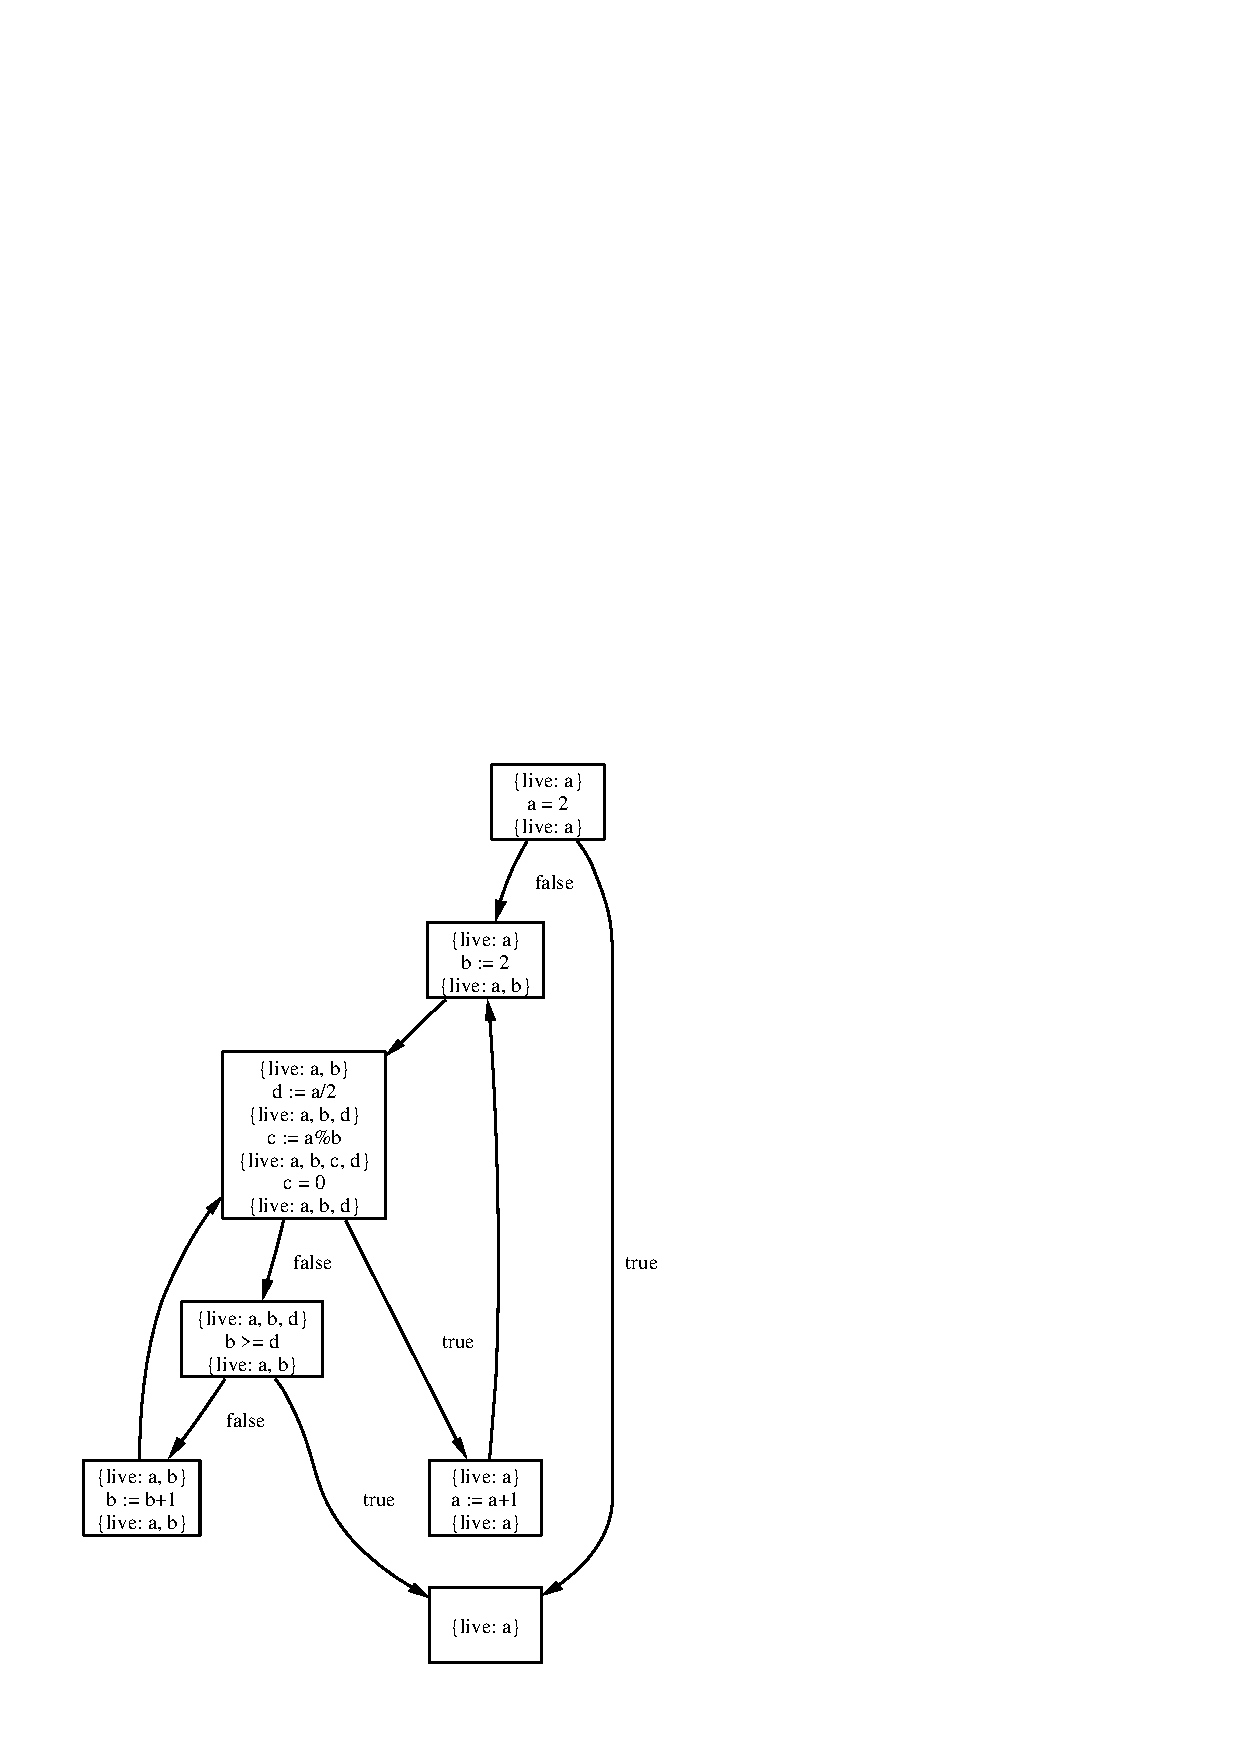
\includegraphics[angle=0]{wasn8-s2}
\end{center}

\item See (a)
\item Assuming \texttt{a} is a natural number greater than 1, this
program computes the smallest prime that is greater than or equal to
\texttt{a}.
\end{enumerate}
\end{enumerate}

\end{document}
